\documentclass[11pt]{article}
\usepackage{listings}
\usepackage{xcolor}
\usepackage{multirow}
\usepackage{multicol}
\usepackage{xparse}
\usepackage{amsmath}
\usepackage[BoldFont]{xeCJK}
\usepackage[most]{tcolorbox}
\usepackage[T1]{fontenc}

\usepackage{lmodern}

\graphicspath{ {./image/} }
\renewcommand\thesection{Question \ \arabic{section}}
\renewcommand\thesubsection{\arabic{section}-(\alph{subsection})}
\usepackage{hyperref}
\hypersetup{
    colorlinks=true,
    linkcolor=blue,
    filecolor=magenta,      
    urlcolor=cyan,
    pdftitle={習題4 },
    pdfpagemode=FullScreen,
}
\usepackage[a4paper, margin={3cm}]{geometry}
\linespread{1.15}
\lstset{language=C,keywordstyle={\bfseries \color{blue}}}
	

\title{習題4 \\\Large 總體經濟學原理與實習}
\author{B10703033\ 財金一\ 邱奕璉
\\ B10703103\ 財金一\ 許羽婷
\\ B10705007\ 資管一\ 劉冠甫
\\ B10705047\ 資管一\ 邱秉辰}
\date{March 25, 2022}

\setlength{\parindent}{0em}
\setlength{\parskip}{0.5em}

\setCJKmainfont{GenRyuMin TW}
\begin{document}



\maketitle

% Question 1
\section{} 
\subsection{}
文中所指的利率為 $0.13\%$

$$
(1.0013)^x = 2 \implies x \approx 534 \ (\text{years})
$$

\subsection{}
$$
(1.008)^x = 2 \implies x \approx 87 \ (\text{years})
$$

\subsection{}
\begin{enumerate}
    \item 儲蓄更少，投入更多在當期的消費支出上
    \item 儲蓄更多，以補足所獲得的利息
    \item 轉向風險更高的投資（如股票等）
\end{enumerate}


\section{}
\subsection{}
第一期之預算限制式為 
$$
b_0(1+R_0) + m_0 + p_1y_1 = p_1c_1+b_1+m_1
$$
其中 
$b_0 = 150\text{萬}, \ m_0 = 2\text{萬}, \ R_0 = 2\%,  \ p_1y_1 = 100\text{萬}, \ p_1c_1 = 60\text{萬},  \ m_1 = 3\text{萬}$

\subsection{}
$$
\text{名目儲蓄} = b_0R_0+p_1y_1 - p_1c_1  = 3+100 - 60 = 43(\text{萬元})
$$

\subsection{}
$$
b_1 = 150(1.02)+2+100-63 = 192(\text{萬元})
$$


\subsection{}
$$
p_1y_1 - p_1c_1 = (b_1+m_1) - (b_0+m_0)  
$$
$$
100 - 60 = (b_1+3) - (0+2)
$$
$$
b_1 = 39(\text{萬元}) 
$$

\subsection{}
因為儲蓄為資產的變動，固定資產投資前後價值不變，因此名目儲蓄仍為43萬元。

\section{}
\subsection{}
$$
b_0(1+ R_0)+p_1y_1+\frac{p_2y_2}{1+R_1} = p_1c_1+\frac{p_2c_2}{1+R_1} 
$$$$
40(1.005)+30+ 0 = c_1 + \frac{c_2}{1.005}
$$
與橫軸焦點的截距：$c_2 = 0 \implies $ 所求 
$$40(1.005)+30 = c_1 = 70.2 =  \text{與橫軸之截距}$$

\begin{figure}[h]
    \centering
    
\includegraphics[scale = 0.4]{3a.png}
\end{figure}

\subsection{}
第一期儲蓄 = $40(0.002)+30 - 40 = -9.2$ \\
$b_1 - b_0 = -9.2 \implies b_1 = 30.8（\text{萬元}） $

\text{since}  $b_2 = 0$,
$$b_2 - b_1 = (b_1(0.002) - c_2)$$
 $$0 - 30.8 = 0.0616-c_2$$
 $$c_2 = 30.8616 (\text{萬元})$$

\subsection{}
新的預算限制線
$$
b_0(1+ R_0)+p_1y_1+\frac{p_2y_2}{1+R_1} = p_1c_1+\frac{p_2c_2}{1+R_1} $$$$
40(1.002)+30+ 0 = c_1 + \frac{c_2}{1.002}
$$

\begin{figure}[h]
    \centering
    
\includegraphics[scale = 0.4]{3c.png}
\end{figure}
利率下降後，所有 $(c_1,c_2)$ 的消費組合有下降的現象，代表購買力下降
\pagebreak
\section{}
\subsection{}
\begin{figure}[h]
    \centering
    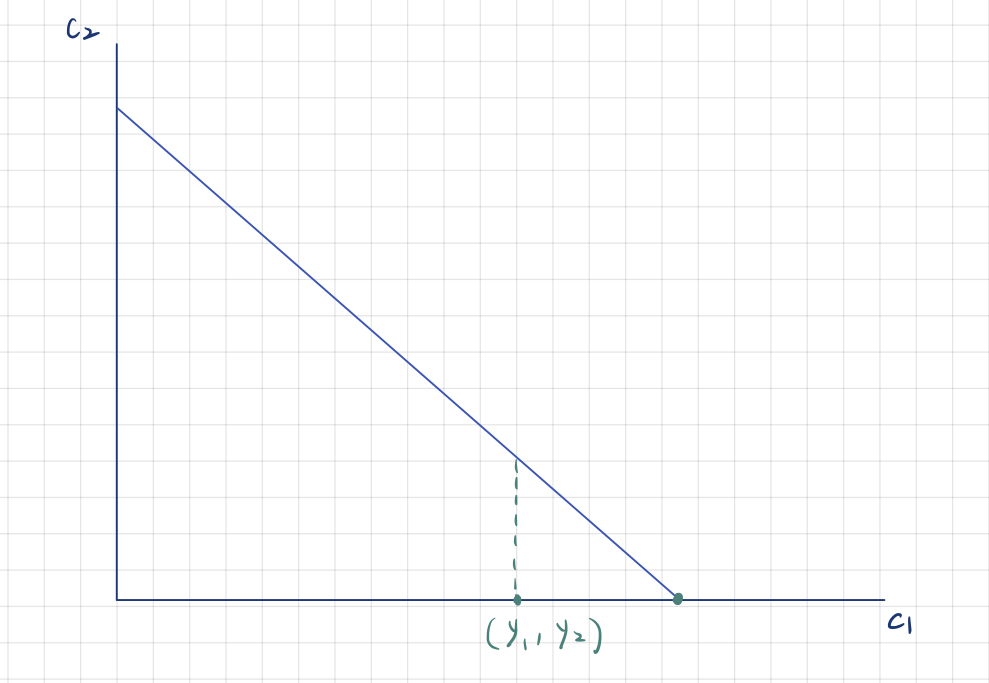
\includegraphics[scale = 0.3]{4a.png}
\end{figure}
\subsection{}
$$
c_2 = \frac{b_0(1+R_0)}{p_1}(1+r_1)
$$

\subsection{}
$$
b_0 < 0 \implies \text{x截距} < y_1
$$

\begin{figure}[h]
    \centering
    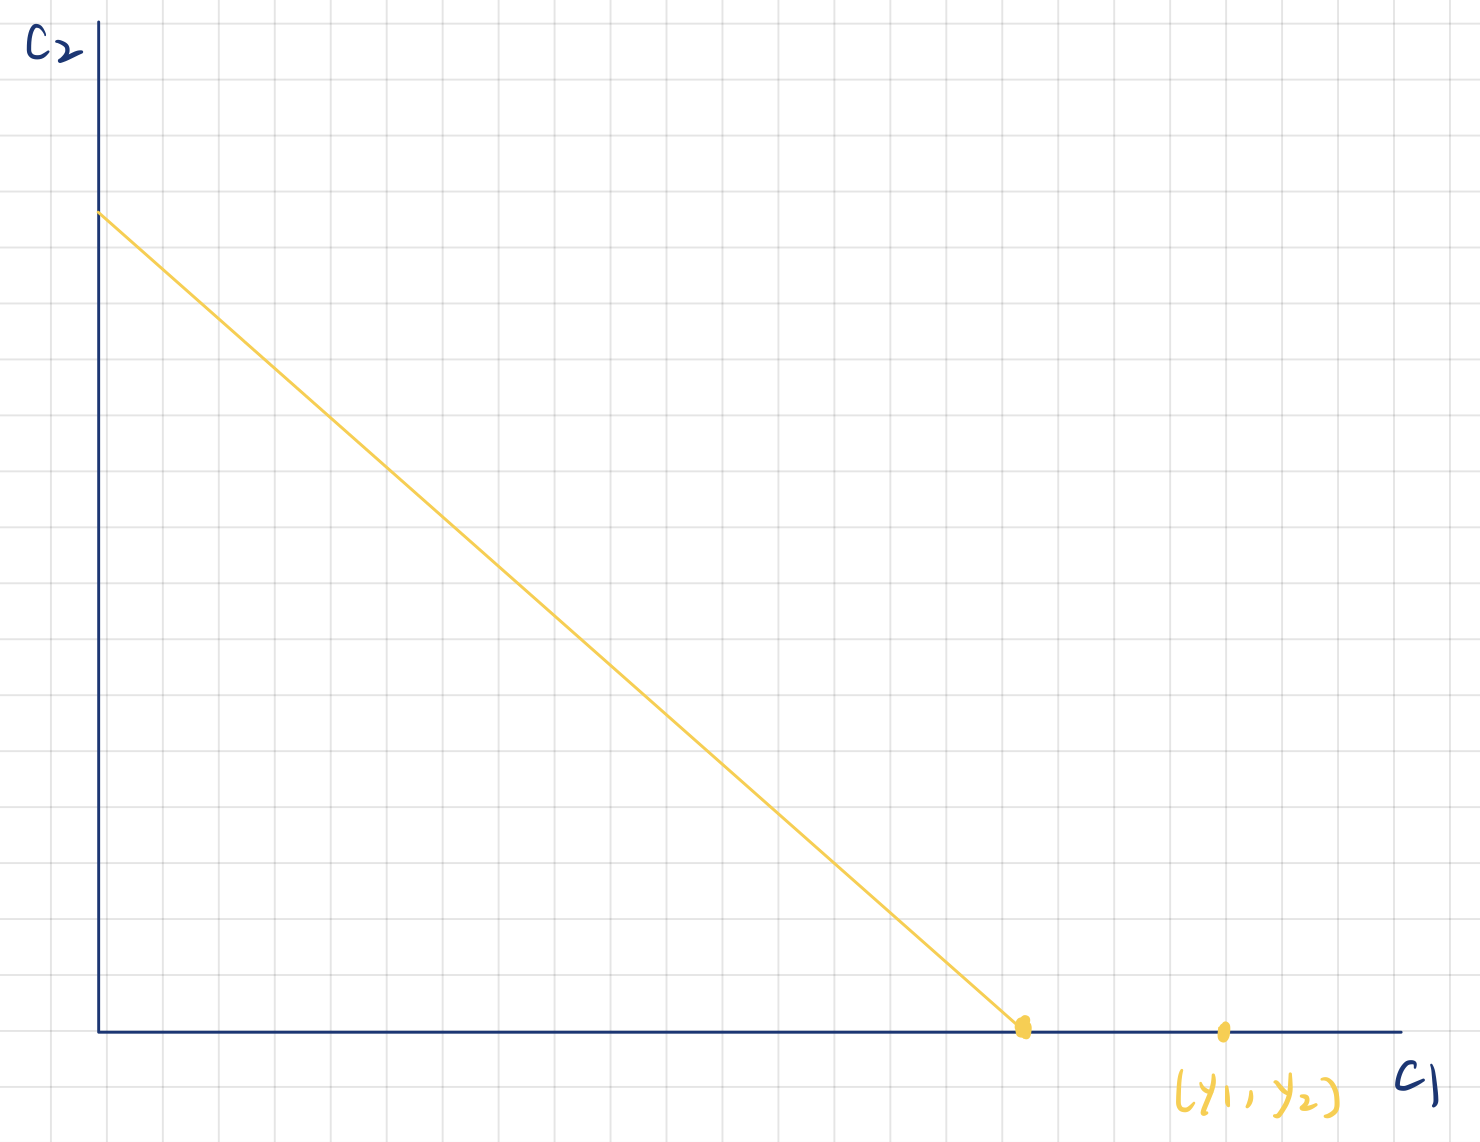
\includegraphics[scale = 0.15]{4c.png}
\end{figure}

由圖，顯然可知 $c_1 = y_1$ 的選擇是不可能的
\pagebreak

\section{}
\subsection{}
Suppose that $b_0=b_2 = 0$, 第一期的預算限制式：
$$
p_1y_1 = p_1c_1+b_1 
$$
第二期的預算限制式：
$$
b_1 + p_2y_2 = p_2c_2 
$$
兩式相加：
$$
p_1y_1+p_2y_2 = p_1c_1+p_2c_2
$$



\subsection{}
Suppose that $b_0=b_2 = 0$, 第一期的預算限制式：
$$
p_1y_1 = p_1c_1+b_1 
$$
第二期的預算限制式：
$$
b_1 + \frac{p_2y_2}{1+R_1} = \frac{p_2c_2}{1+R_1} 
$$
兩式相加：
$$
p_1y_1+\frac{p_2y_2}{1+ R_1} = p_1c_1 +\frac{p_2c_2}{1 + R_1}
$$

\begin{figure}[h]
    \minipage{0.5 \textwidth}
    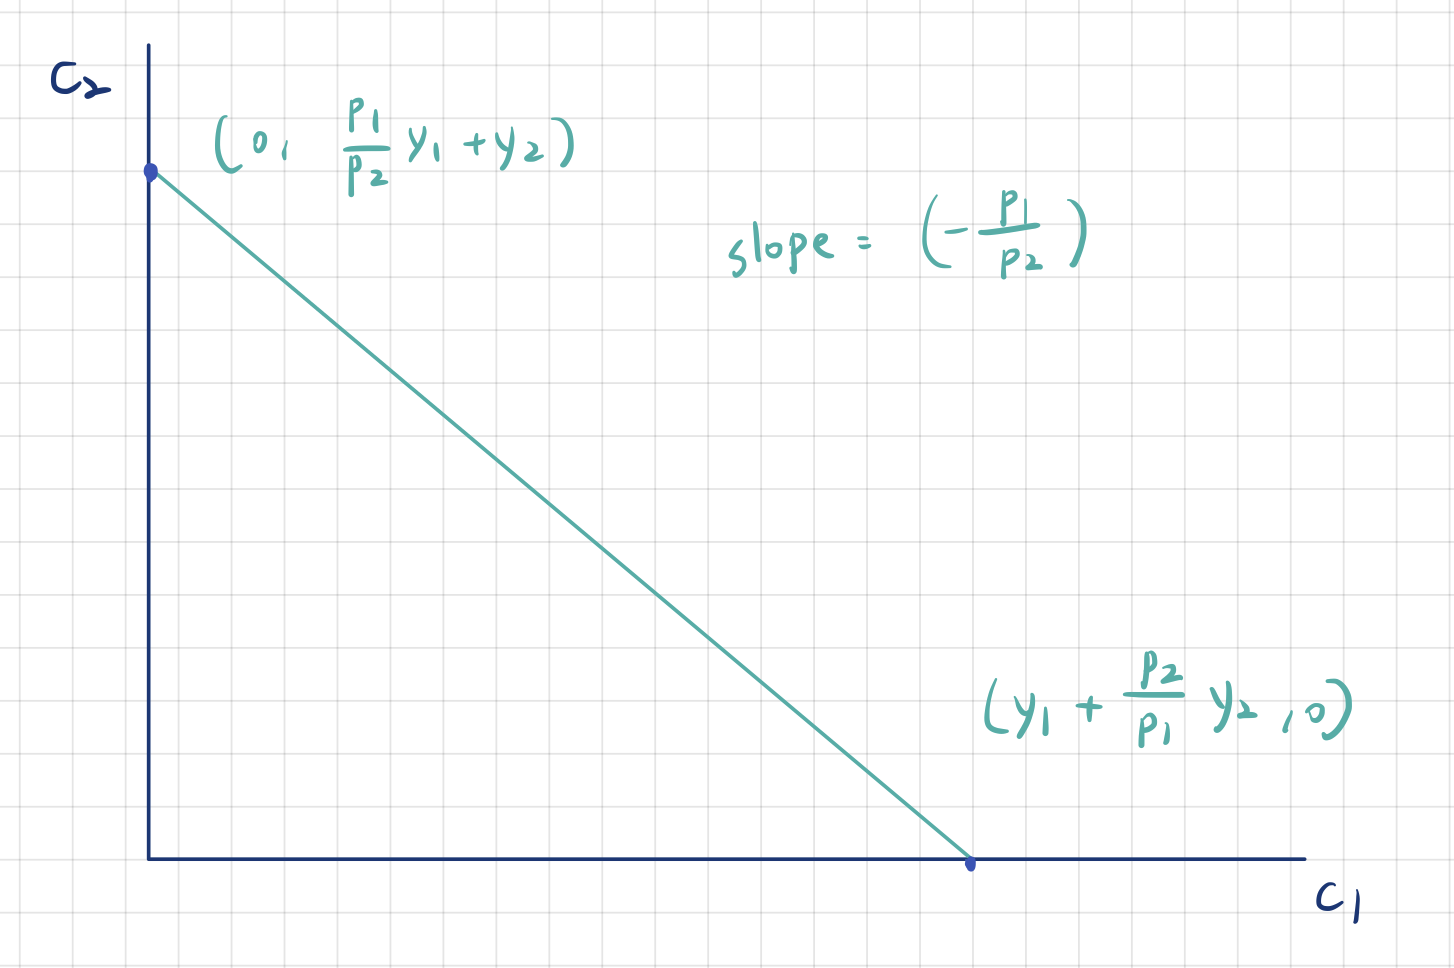
\includegraphics[scale = 0.15]{5a.png}
    \caption{5(a)之作圖}
    \endminipage
    \minipage{0.5 \textwidth}
    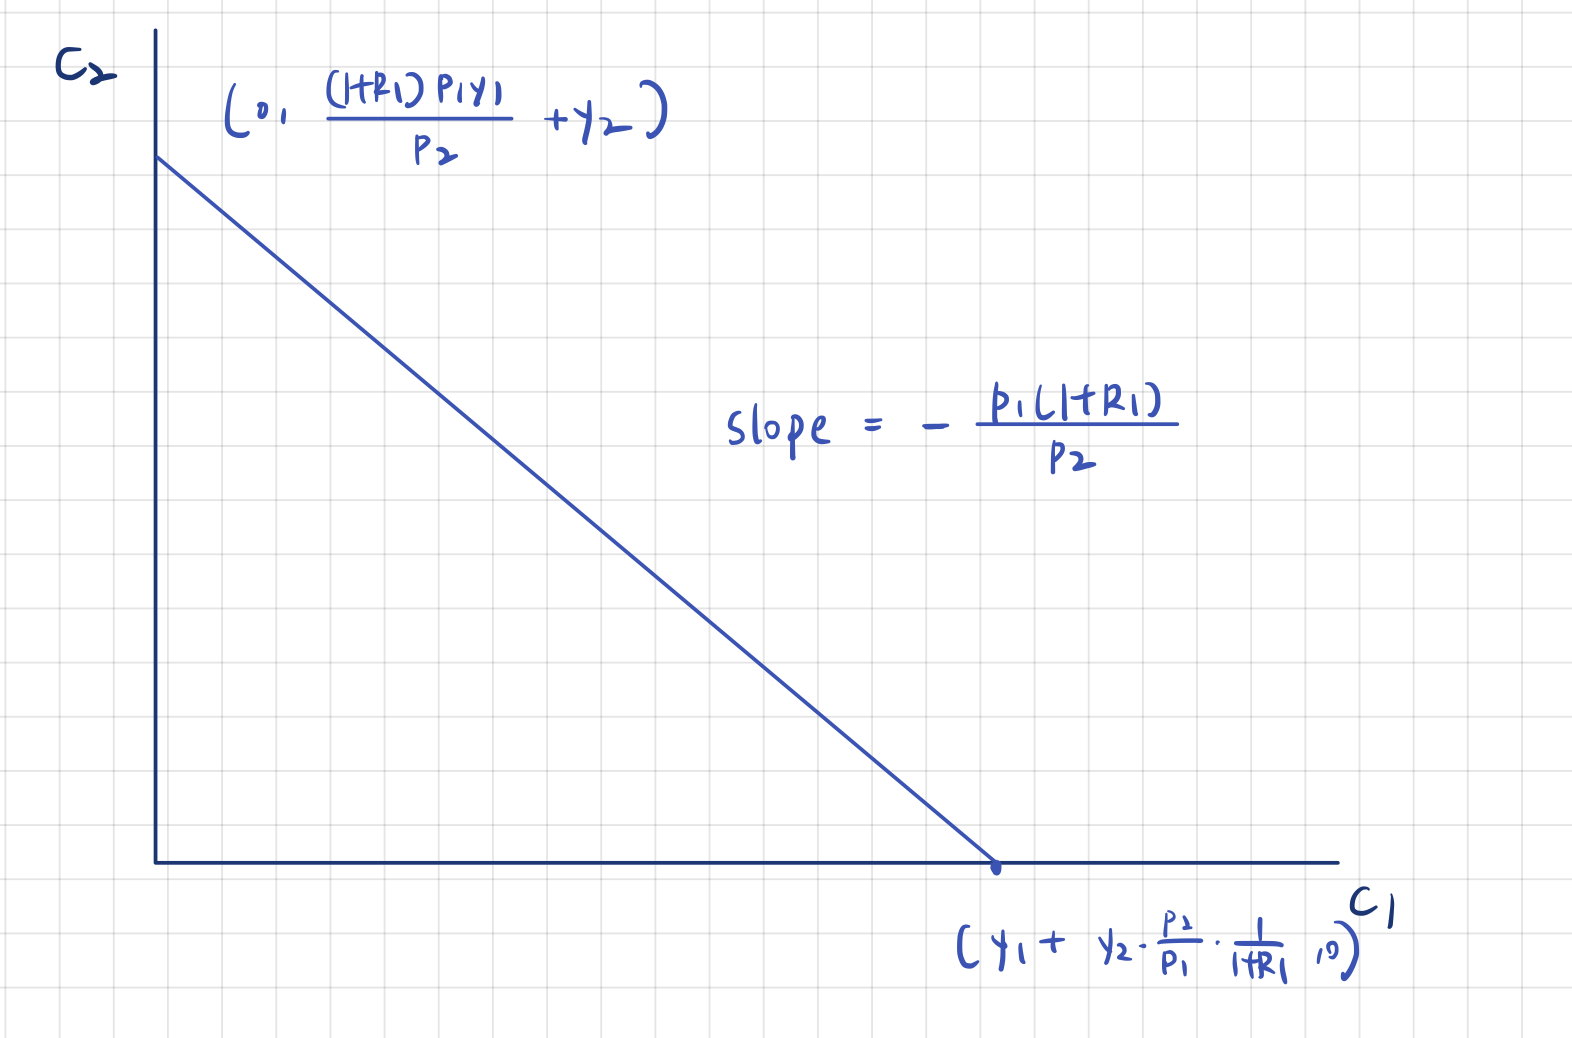
\includegraphics[scale = 0.15]{5b.png}
    \caption{5(b)之作圖}
    \endminipage 
\end{figure}


\end{document}
